\documentclass[11pt,twoside]{article}

\usepackage{amsmath}
\usepackage{graphicx,epsfig}
\usepackage{graphicx}
\usepackage{amsmath,amssymb,amsbsy,bm}
%\usepackage[framed]{mcode}

\newlength{\toppush}
\setlength{\toppush}{2\headheight}
\addtolength{\toppush}{\headsep}

\renewcommand{\bottomfraction}{0.95}

\newcommand{\htitle}[3]{\begin{center}
\vspace*{-\toppush}
{\large MASSACHUSETTS INSTITUTE OF TECHNOLOGY}\\
{\small Department of Electrical Engineering and Computer Science}\\
\vspace*{1ex}{\Large #2}\end{center}
\noindent
\newline\parbox{6.5in}
{Fall 2013\hfill Issued : #1 \newline
 Problem Set 3 \hfill Due : #3\newline
%\profs \hfill %Handout #1\vspace*{-.5ex}\newline
%\mbox{}\hrulefill\mbox{}
}}

\newcommand{\mcO}{\mathcal{O}}
\newcommand{\handout}[3]{\thispagestyle{empty}
\pagestyle{myheadings}\htitle{#1}{#2}{#3}}

\setlength{\oddsidemargin}{0pt}
\setlength{\evensidemargin}{0pt}
\setlength{\textwidth}{6.5in}
\setlength{\topmargin}{0in}
\setlength{\textheight}{8.5in}


\newcommand{\pp}[2]{\frac{\partial #1}{\partial #2}}%
\newcommand{\ppp}[2]{\frac{\partial^2 #1}{\partial #2^2}}%
\newcommand{\dd}[2]{\frac{d #1}{d #2}}%
\newcommand{\ddd}[2]{\frac{d^2 #1}{d #2^2}}%
\newcommand{\matend}{\end{array}\right]}
\newcommand{\matc}{\left[\begin{array}{c}}
\newcommand{\matcc}{\left[\begin{array}{cc}}
\newcommand{\bb}{\mathbf{b}}
\newcommand{\bx}{\mathbf{x}}
\newcommand{\bA}{\mathbf{A}}
\newcommand{\DD}[2]{\frac{D #1}{D #2}}%
\newcommand{\Uvec}{\mathbf{U}}
\newcommand{\uvec}{\mathbf{u}}
\newcommand{\tauvec}{\bm{\tau}}
\newcommand{\omegavec}{\bm{\omega}}


\renewcommand{\Re}{\mathrm{Re}}


\begin{document}


\handout{Sept 18, 2013}{6.301 Solid State Circuits}{Sept 25, 2013}
\setlength{\parindent}{0pt}

\newcommand{\solution}{
 \medskip
 {\bf Solution:}
}

\hrulefill

\flushleft

\subsection*{Problem 1: Cascades}
	For the following circuits find the midband gain, input impedance (not including $R_s$), and output impedance in terms of transistor small-signal parameters ($r_\pi$, $gm$, etc.) and labeled components. Assume $r_o=\infty$.
\begin{enumerate}
	\item[(a)] Cascaded common emitter (CE-CE) amplifier:

\begin{center}
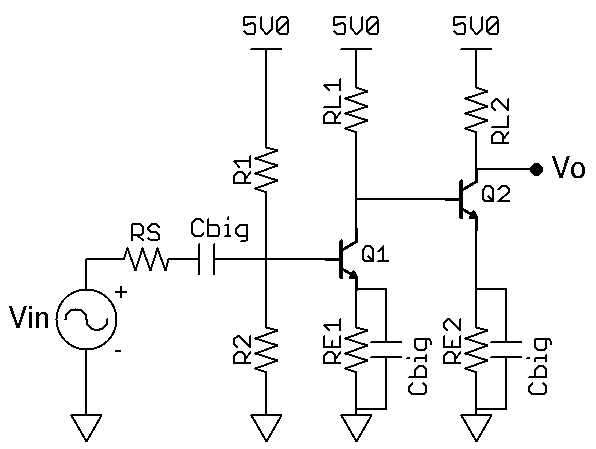
\includegraphics[width=0.5\textwidth]{ce-ce.png}
\end{center}
	\item[(b)] Cascaded common source (CS-CS) amplifer:
\begin{center}
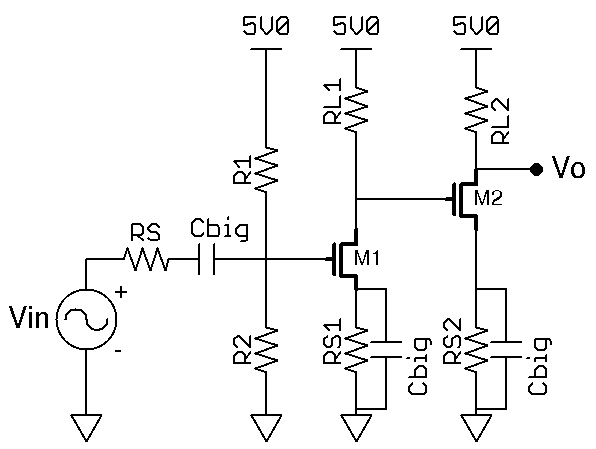
\includegraphics[width=0.5\textwidth]{cs-cs.png}
\end{center}
\end{enumerate}
\clearpage

\subsection*{Problem 2: Three transistor cascade}
	Consider this common emitter-emitter follower-common emitter (CE-EF-CE) amplifier:
\begin{center}
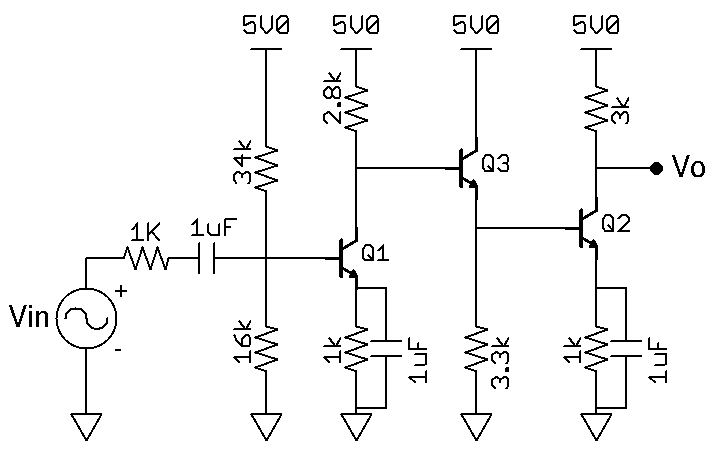
\includegraphics[width=0.6\textwidth]{ce-ef-ce.png}
\end{center}
\begin{enumerate}
	\item[(a)] Find the midband gain, input impedance, output impedance, and power dissipation, assuming $\beta=200$, $V_{BE}=0.6V$, and $r_o=\infty$
	\item[(b)] What is the largest AC input amplitude, $v_{in}=A\sin(t)$ that does not push any transistor into saturation
	\item[(c)] Find the value of $R_{L_2}$ that permits the largest output swing
	\item[(d)] Find the value of $I_{C_2}$ (via modifying $R_{E_2}$) that permits the largest output swing
	\item[(e)] Find the new midband gain in (c) and (d)
\end{enumerate}

\subsection*{Problem 3: Looking at limits}
	\item[(a)] For the common emitter amplifier below find the maximum midband gain, $a_v$, in terms of $V_{CE_{sat}}$, $V_{BE}$, and any labels in the schematic. 

\begin{center}
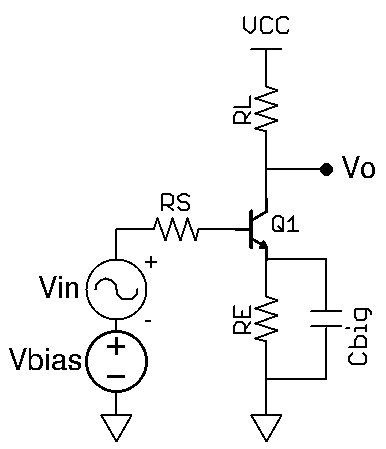
\includegraphics[width=0.35\textwidth]{ce-max.png}
\end{center}

	\item[(b)] What is the maximum output swing (before saturating) for an amplifier configured with maximum midband gain?
	\item[(c)] Given an AC input that is symmetric about ground, find the midband gain that permits the maximum output swing.


\subsection*{Problem 4: More transfer function review}
	For the following transfer functions find the 3 dB bandwidth (the frequency at which the magnitude of the frequency response is .707 of the DC gain) in hertz.  For $A_1$, $A_2$, and $A_4$ find the 10-90\% risetime.\\
\begin{equation*}
 A_1(s) = \frac{1}{\tau s+1} \quad A_2(s)= \frac{10}{(\tau s+1)^2} 
\end{equation*}
\begin{equation*}
 A_3(s) = \frac{100}{(\tau s+1)^M} \quad A_4(s)= \frac{\omega_n^2}{s^2+2\zeta\omega_n s+\omega_n^2} 
\end{equation*}

\subsection*{Problem 5: Frequency Domain Jungle Gym}
	For the following transfer functions, sketch the pole-zero plot, the bode plot, and the step response.
\begin{equation*}
 A_1(s) = \frac{1}{s^2} \quad A_2(s) = \frac{20}{s^2+2s+1} \quad A_3(s) = \frac{10}{s^2+s+1}
\end{equation*}
\begin{equation*}
 A_4(s) = \frac{s+1}{s+2} \quad A_5(s) =  \frac{s+2}{s+1} \quad A_6(s) = \frac{s-1}{s+1}
\end{equation*}

\end{document}
